\chapter{Introduzione}
Al giorno d'oggi l'utilizzo della voce per automatizzare i processi della vita quotidiana si sta sempre più espandendo, dall'assistente vocale nella propria casa a quello nel proprio cellulare. Sono sempre stato incuriosito da questo tipo di tecnologie e il tirocinio era il modo migliore per comprendere lo sviluppo di software di questo tipo. Il progetto mi è stato proposto dall'azienda fiorentina E.D.P. Service, società collegata al gruppo Best Vision Holding, il cui scopo era integrare una funzionalità nuova nel sito del cliente BPS(suisse) che permettesse di eseguire pagamenti o trasferimenti di denaro usando linguaggio naturale comunicando direttamente con l'applicazione.
I pagamenti compiuti tramite la piattaforma web utilizzano la classica procedura di compilamento manuale di alcuni campi di testo, come ad esempio la quantità di denaro da trasferire e l'iban del conto del destinatario.
Software di questo tipo si suddividono in 2 parti: una parte adibita all'interazione utente definita interfaccia grafica o frontend, e la parte che gestisce le informazioni chiamata backend o lato server.
\iffalse
https://it.wikipedia.org/wiki/Front-end\_e\_back-end
\fi
La parte del frontend gestisce principalmente le modalità di accesso dell'utente consentendogli di interagire con l'applicativo eseguendo le azioni messe a disposizione, come ad esempio: visualizzare il numero di transazioni eseguite, creare un pagamento, controllare l'andamento del mercato in base a una determinata valuta.
Per riuscire a sviluppare un'integrazione in questo sistema ho studiato i linguaggi usati dalla piattaforma della banca, principalmente formata da codice HTML, CSS, e AngularJS.
L'ultimo citato è un web-framework di casa Google scritto in JavaScript che permette di dinamicizzare una pagina web utilizzando dei comandi a livello di codice HTML, chiamati direttive, che vengono poi eseguiti da AngularJs una volta che la pagina web viene caricata dal browser.
Tutto ciò che riguarda il lato server: gestione, elaborazione e immagazzinamento dei dati forniti dal frontend viene eseguita dal backend, parte fondamentale di un servizio web bancario che deve garantire sicurezza e reperibilità dei dati. Il backend sviluppato da Best Vision è diviso in un servizio di database e uno di gestione del database scritto per intero in linguaggio Java usando il framework Spring.
Inserire una funzionalità che permettesse di eseguire queste azioni usando la sola voce avrebbe diminuito il numero di azioni che l'utente avrebbe dovuto eseguire per ottenere ciò che cercava, dovevo quindi imitare il comportamento umano di un operatore di banca. Per fare questo è stato pensato di sviluppare un servizio di chat bot che riuscisse a comprendere il linguaggio naturale umano e producesse una risposta in completa autonomia eseguendo le azioni necessarie richieste dall'utente.
Il pagamento tramite chat doveva quindi eseguire tutte le richieste al server nel giusto ordine prima di completare la transazione voluta: autorizzazione per accedere al conto dell'utente, richiesta di trasferimento di capitale verso terzi e delega della conferma del transazione.
Nel mio caso il frontend è rappresentato dalla chat in cui l'utente può decidere se scrivere un testo con linguaggio naturale oppure utilizzare il servizio vocale, il backend invece è composto da un'intelligenza artificiale che genera una risposta e agisce in base alle richieste.
Quando un utente invia un messaggio si aspetta che venga generata una risposta consona, cioè venga eseguita una analisi del testo e formulata una frase di senso compiuto che riesca a rispondere in maniera corretta al messaggio inviato.
L'analisi del testo viene definita comprensione del linguaggio naturale, in inglese Natural Language Understanding (NLU), cioè attribuire alla frase analizzata un intento e estrarre da essa oggetti che possono essere utili per la generazione di una risposta.
L'effettiva generazione della risposta però non è un compito che viene esercitato dal NLU, ma da un Natural Language Generator (NLG) che in base all'analisi precedente riesca a determinare la miglior risposta possibile.
\begin{figure}[H]
 \centering
    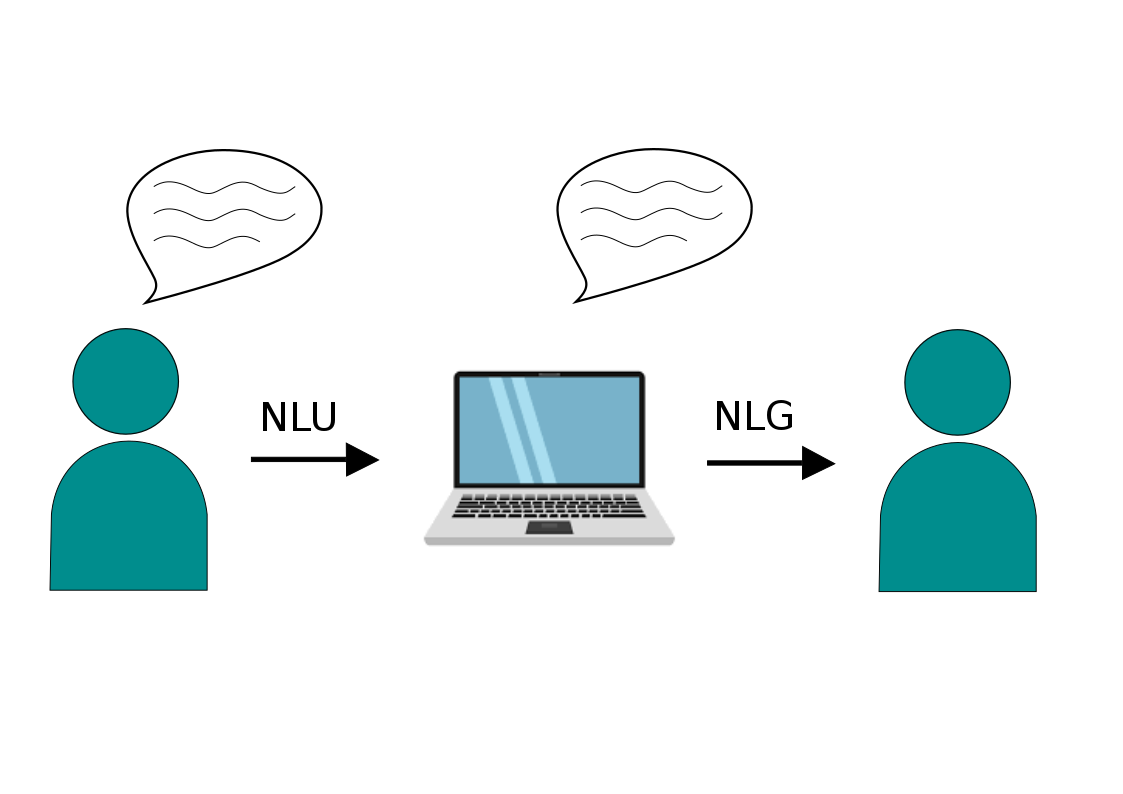
\includegraphics[width=0.4\textwidth]{img/nlu_nlg.png}
 \caption{Chat prototype}
\end{figure}
Il chatbot voluto è quindi formato dalla chat e 2 tipi di intelligenza artificiale: una che esegue il NLU e un'altra che racchiuda il compito di NLG.
\iffalse
https://en.wikipedia.org/wiki/Natural-language_understanding
https://www.expertsystem.com/natural-language-understanding-different-nlp/
https://rasa.com/
https://rasa.com/docs/get\_started\_step1/
https://www.techopedia.com/definition/33013/natural-language-understanding-nlu
https://www.sisense.com/glossary/natural-language-understanding/
\fi
Per la creazione del bot ho usato una libreria open source sviluppata in Python chiamata \textbf{Rasa}, che mette a disposizione tutti gli strumenti che servono per poter sviluppare intelligenze artificiali di questo tipo. I tools che ho usato sono: rasa\_nlu e rasa\_core, il primo per eseguire il compito di NLU e l'altro quello di NLG eseguendo anche le azioni necessarie.
La corretta esecuzione degli strumenti appena descritti si basa su modelli generati grazie a dataset precedentemente realizzati, i quali contengono veri e propri esempi di frasi e possibili conversazioni che l'utente potrebbe usare.
Teoricamente questo tipo di processo richiederebbe un numero molto elevato di esempi per essere più preciso, in questo caso però mi è bastato creare un dataset con una popolazione di soli 60 esempi per ottenere un prototipo di bot ragionevolmente preciso. 
Completato lo sviluppo delle 2 intelligenze artificiali queste sono state collocate in un server dove potessero rimanere in ascolto di tutti i messaggi da parte dei clienti.
L'ultimo passo è stato quello di integrare il prototipo della chat nel sito web di BPS(suisse) attuando alcune modifiche sia lato backend, in cui sono state aggiunte alcune proprietà per rendere il server più sicuro, sia lato frontend, modificando la web application includendo la chat da me creata.
Questo ha completato il lavoro di tirocinio consentendo all'azienda di inserire nella fase di produzione e miglioramento l'integrazione da me sviluppata.
\begin{figure}[H]
 \centering
    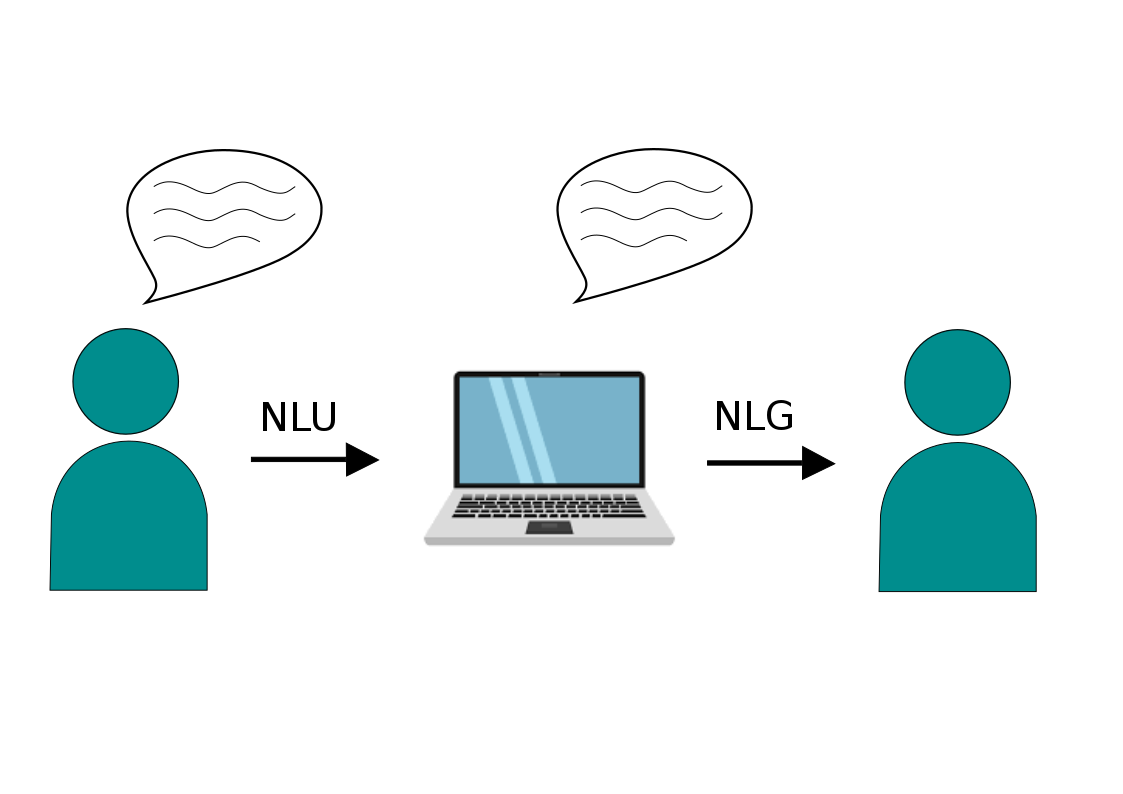
\includegraphics[width=0.4\textwidth]{img/nlu_nlg.png}
 \caption{Chat prototype}
\end{figure}

\iffalse
<frase iniziale>
<perchè ho scelto questa tesi>
<perchè edp ha scelto questo percorso>
<che progetto è?>
<spiegazione generica degli elementi fondamentali del progetto>
<definizione di un percorso iniziale>
<spiegazione dell'architettura del software di BPS(swisse)>
<studio della libreria principale usata dal frontend del software>
<studio degli elementi principali per la creazione del frontend ----> chat di testo>
<creazione della chat e test del prototipo usando sia testo che voce>
<studio di una possibile implementazione del backend di nlu>
<perchè è stato scelto di non usare dialogflow>
<passaggio a RASA>
<sviluppo del primo modello usato per il NLU>
<creazione del server rasa>
<refactor chat>
<perfezionamento del modello di NLU>
<integrazione>
<problemi affrontati durante l'integrazione>
<conclusione introduzione>
\fi
